
\documentclass[11pt,    % schriftgr��e 11
               twoside, % doppelseitige Seiten
               a5paper, % A5, statt amerikanisches letter-format
               parskip=half
               ]{scrartcl}
               
\usepackage[latin1]{inputenc}  % eingabecodierung um deutsche Sonderzeichen 
                               % nat�rlich eingeben zu k�nnen ���
\usepackage[T1]{fontenc}
\usepackage{lmodern}
\usepackage[ngerman]{babel}
\usepackage{xcolor}

\usepackage{microtype}

\usepackage{ifthen}     % conditional 
\usepackage{url}        % provides \url command
\usepackage{graphicx}   % f�r bilder
\graphicspath{{../../art/}}   % suchpfad f�r bilder
                        % damit reicht \includegraphic{bild},
                        %        statt \includegraphic{pic/bild} 
                        %  prektisch f�r low und hi-res varianten
 

%\usepackage{amsmath} % mathematik befehle
%\usepackage{amssymb} % mathematik symbole

\usepackage{paralist}  % compact enums and lists
\usepackage{array}     % stellt den Befehl \newcolumntype bereit 
\usepackage{colortbl}  % farbliche Tabellen
\newcolumntype{C}[1]{>{\centering}p{#1}} 
\newcolumntype{L}[1]{>{\raggedright}p{#1}} 
\newcolumntype{R}[1]{>{\raggedleft}p{#1}} 



\usepackage{geometry}           % erweiterte Seitengeometriefunktionen
\usepackage[automark]{scrpage2} % Koma Seitenstile


% Dieses File nicht direkt editieren - wird aus 'srclatexBridge.tex' erzeugt.
%%%%%%%%%%%%%%%%%%%%%%%%%%%%%%%%%%%%%%%%%%%%%%%%%%%%%%%%%%%%%%%%%%%%%%%%%%%%%%%%%%%%%%%%%%%%%%%%%%%%%%%%%%
%%% THIS FILE IS AUTOMATICLY GENERATED - DO NOT CHANGE THINGS HERE - THEY WILL BE OVERWRITTEN             
%%% Please edit  'srclatexBridge.tex' 
%%% and execute 'latex_Preprocess.pl' again.
%%%%%%%%%%%%%%%%%%%%%%%%%%%%%%%%%%%%%%%%%%%%%%%%%%%%%%%%%%%%%%%%%%%%%%%%%%%%%%%%%%%%%%%%%%%%%%%%%%%%%%%%%%

















































% this file contains some c-style preprocessor makros to support
% individual generation of the manual depending on software configuration
%
% use the perl script 'latex_Preprocess.pl' that also resides in this directory
% adapt it to your environment (pdflatex path, gcc command) first









% wird hier definiert, wegen optionaler Paketoption ^^
\usepackage[ %
            bookmarksopen,%
            bookmarksopenlevel = 3,%
            bookmarksnumbered,%
            pdftitle={Word Clock Benutzerhandbuch},%
            pdfsubject={},%
            pdfcreator={PDF-LaTeX mit TeXnicCenter und HyperRef},%
            pdfauthor={Rene Staffen},%
            pdfproducer={Rene Staffen},%
            pdfstartview = FitH%
%,draft %disables links and draws link text normaly black
           ]{hyperref}


\newcommand{\numberToText}[1]{\ifthenelse{#1=1}{ein }{%
\ifthenelse{#1=2}{zwei }{%
\ifthenelse{#1=3}{drei }{%
\ifthenelse{#1=4}{vier }{%
\ifthenelse{#1=5}{f�nf }{%
\ifthenelse{#1=6}{sechs }{%
\ifthenelse{#1=7}{sieben }{%
\ifthenelse{#1=8}{acht }{%
\ifthenelse{#1=9}{neun }{%
\ifthenelse{#1=10}{zehn }{%
}}}}}}}}}}}






\newcommand{\WCmonocolor}{0}


\newcommand{\WCindividualCfg}{0}
\newcommand{\WCautoSave}{1}
\newcommand{\WCdcf}{1}
\newcommand{\WCambilight}{1}
\newcommand{\WCbluetooth}{1}
\newcommand{\WCauxIO}{1}


\newcommand{\WCcolorProfiles}{\numberToText{4}}

\newcommand{\WCSoftWareVersion}[2]{#1.#2} % Sofftwareversionen zusammensetzen (aus defines)
\newcommand{\SoftwareVersion}{\WCSoftWareVersion{0}{12}}
  % bindet auch hyperref mit ein


\geometry{a5paper,left=22mm,right=22mm, top=25mm, bottom=3cm}


\setlength{\tabcolsep}{5pt}
\setlength{\extrarowheight}{0pt}

%\setlength{\parskip}{1.5ex}  % Abstand zwischen Abs�tzen
%\setlength{\parindent}{0em}  % kein Einzug bei neuen Abs�tzen


% umgebung f�r Anmerkungen defnieren
\newenvironment{Anmerkung}{\par\begin{itshape}\underline{Anmerkung:}\\}{\end{itshape}}



\definecolor{colorBack}{rgb}{.58,.21,.20}
\definecolor{sectionColor}{rgb}{0.31,0.51,0.74}


\newcommand{\normalModeName}{\ifthenelse{\WCindividualCfg=0 \or \WCmonocolor=0}{Ein\-farb-Mo\-dus}{Stan\-dard-Mo\-dus}}


%% define Pagestyle
%\addtokomafont{pagenumber}{\color{white}}
%\newcommand{\HeadBox}[1]{  \colorbox{colorBack}{\hfill\textcolor{white}{#1}\hfill}}
%\newenvironment{HeadBox}{
% \def\FrameCommand{\fboxsep=1cm \colorbox{colorBack}}
%  \MakeFramed {\advance\hsize-1.1\width\FrameRestore}}
%{\endMakeFramed}

\pagestyle{scrheadings}
%\ohead{\HeadBox{\today}}
%\ofoot{\HeadBox{\pagemark}}
\ohead{\today}
\chead{[Word Clock]}
\cfoot{\headmark}
\ofoot{\pagemark}
\setheadsepline{.4pt}
\setfootsepline{.4pt}
%% end define Pagestyle

\addtokomafont{section}{\color{sectionColor}\mdseries}
\addtokomafont{subsection}{\color{sectionColor}\mdseries}
\addtokomafont{subsubsection}{\color{sectionColor}\mdseries}





\begin{document}





%% Deckblatt

\begin{titlepage}
\pdfbookmark[0]{WordClock}{toc}

\begin{addmargin}{-1cm}

\begin{center}

%\vspace*{1cm}
\vfill

\includegraphics[width=1.2\textwidth]{wordclockFront_Manual_ger.pdf}

\vfill

\large
Benutzerhandbuch\\[0.1\baselineskip]
zu Software v\SoftwareVersion
\vfill

\end{center}
\end{addmargin}

\clearpage

\vfill

Projektteam:
\begin{list}{}{}
	\item Frank Meyer (ukw)
	\item Ren� Staffen (vladtepesch)
	\item Torsten Giese (wawibu)
	\item Rene H (promeus)
	\item Simon Mahler (edimahler) 
\end{list}

\vfill


% liste darf nicht leer sein, daher diese Abfrage
\ifthenelse{ \WCindividualCfg=0 \or \( \WCbluetooth=1 \or \WCdcf=1 \or \WCmonocolor=0 \or \WCambilight=1\) }
{
Besondere Eigenschaften:
  
  \begin{list}{\ifthenelse{\WCindividualCfg=1}{$\bullet$}{[~~~]} }{}


   \ifthenelse{\WCindividualCfg=0 \or \WCmonocolor=0}
      {\item RGB (Mehrfarb-LEDs)}{}
      
   \ifthenelse{\WCindividualCfg=0 \or \WCambilight=1}
      {\item Ambilight (Umgebungslicht)}{}
      
   \ifthenelse{\WCindividualCfg=0 \or \WCdcf=1}
      {\item Funkuhr-Empf�nger}{}
      
   \ifthenelse{\WCindividualCfg=0 \or \WCbluetooth=1}
			{\item Bluetooth}{}
			
  \end{list}
}
{}

\vfill


\end{titlepage}



\clearpage
\linespread{1.0} % Zeilenabstand 1,0
% Inhaltsverzeichnis	
	\pdfbookmark[1]{\contentsname}{toc}\tableofcontents
%	\input{diplomarbeit.toc}
%\tableofcontents



\clearpage

\section{Inbetriebnahme der Uhr}\label{sec_inbetriebnahme}
		
		Die Steuerung der Uhr erfordert eine Infrarot"=Fernbedienung.
		
		Es wird eine Vielzahl von Protokollen unterst�tzt, 
		so dass eine (beinahe) beliebige, �berfl�ssige Fernbedienung benutzt werden kann. 

		Nach Anschluss der Uhr an die Stromversorgung, blinken die vier Minutenpunkte f�r einige Sekunden. 
		
		Anschlie�end wechselt die Uhr in den \normalModeName. 

\clearpage
\section{Antrainieren einer Fernbedienung}\label{sec_trainIr}
		Wird nach einem Neustart der Uhr, w�hrend des Blinkens der Minutenpunkte, 
		ein Infrarot"=Fernbedienungs"=Kommando erkannt, 
		wechselt die Uhr automatisch in den Fernbedienungs"=Trainingsmodus. 
		Nun m�ssen nacheinander allen Kommandos die gew�nschten Fernbedienungstasten 
		zugewiesen werden. 
		
		Soll ein oder mehrere Kommandos nicht zugewiesen werden,
		\ifthenelse{\WCindividualCfg=1}{
		  da diese nicht ben�tigt werden,	
		}{
			weil zum Beispiel keine Funkuhr-Funktion oder kein Ambilight enthalten ist, 
			oder nur einfarbige LEDs (kein RGB) verwendet werden, 
		}
		kann die Option mit erneutem Druck auf die an/aus-Taste �bersprungen werden.		
		Die �bersprungene Option steht dann sp�ter nicht zur Verf�gung, 
		kann jedoch in einer weiteren Anlernprozedur nach einem Neustart wieder aktiviert 
		werden. 
		
		Die Stundenw�rter zeigen an, welches Kommando nun einer Fernbedienungstaste
		zugewiesen werden soll. 
		Nach dem zw�lften Kommando beginnt die Anzeige der Stundenw�rter wieder bei eins.  
		
		\begin{Anmerkung}
				Eine �bersicht �ber die Kommandos und deren Reihenfolge 
				befindet sich am Ende dieses Kapitels.
		\end{Anmerkung}
		
		
		\begin{Anmerkung}
				Aufgrund der Vielzahl an Herstellern von fernbedienbaren Ger�ten 
				existiert eine ebenso gro�e Vielzahl von Fernbedienungsprotokollen. 
				Es wurde versucht, die h�ufigsten Protokolle zu 
				implementieren. Aufgrund der Vielfalt an 
				unterschiedlichen Fernbedienungsprotokollen, kann es 
				vorkommen, dass nicht alle Fernbedienungen erkannt 
				werden. \\
				Sollte w�hrend des Anlernens der Fernbedienung auffallen, 
				dass die Uhr nicht wie erwartet reagiert 
				(die Zahlenanzeige �berspringt Zahlen oder eine Taste wird 
				erst nach mehrmaligen Dr�cken erkannt), 
				kann das Protokoll der verwendeten Fernbedienung nicht 
				problemlos erkannt werden. 
				In einem solchen Fall, ist die Uhr vom Strom zu trennen und 
				mit einer anderen Fernbedienung neu zu beginnen. 
		\end{Anmerkung}


		\subsection{�bersicht der m�glichen Kommandos}
		\begin{minipage}{\textwidth}
		\newcounter{ircmdNumber} 
		\newcommand{\ircCmdTableLine}[1]{  {\stepcounter{ircmdNumber}\theircmdNumber.}& {#1}&{}\tabularnewline\hline}
		\begin{center}
		   % \footnotesize
			  \arrayrulecolor{colorBack}
				\begin{tabular}{|R{.05\textwidth}L{.6\textwidth}|L{.25\textwidth}|}
						\hline
						\rowcolor{colorBack}  {\textcolor{white}{Nr.}} 
																& {\textcolor{white}{Kommando}} 
																& {\textcolor{white}{Taste eigene Fernbedienung}} 
																\tabularnewline\hline
						\ircCmdTableLine{ein/aus}
						\ircCmdTableLine{heller}
						\ircCmdTableLine{dunkler}
						\ircCmdTableLine{rauf/+}
						\ircCmdTableLine{runter/-}
						\ircCmdTableLine{manuelle Zeiteingabe}
						\ircCmdTableLine{Eingabe der Ein-/Ausschaltzeit}
						\ifthenelse{\WCindividualCfg=0 \or \WCdcf=1}{
							\ircCmdTableLine{Funkuhr-Abgleich manuell starten}
						}{}
						
      			\ircCmdTableLine{\normalModeName \ifthenelse{\WCindividualCfg=0 \or \WCmonocolor=0}{/Farbprofile aktivieren}{}}
      			\ircCmdTableLine{Pulsierender Modus}
      			\ircCmdTableLine{Demo-Modus}
		        \ifthenelse{\WCindividualCfg=0 \or \WCmonocolor=0}{
		      			\ircCmdTableLine{Automatischer Farbwechselmodus (Regenbogen)}
		      			\ircCmdTableLine{Farbe Rot �ndern}
		      			\ircCmdTableLine{Farbe Gr�n �ndern}
		      			\ircCmdTableLine{Farbe Blau �ndern}
		      			\ircCmdTableLine{Farben durchschalten (Regenbogen/Hue)}
						}{}
      			\ircCmdTableLine{aktuelle Helligkeit �bernehmen}
						\ifthenelse{\WCindividualCfg=0 \or \WCambilight=1}{ 
		      			\ircCmdTableLine{Ambilight ein-/ausschalten}
		        }{}
						\ifthenelse{\WCindividualCfg=0 \or \WCbluetooth=1}{ 
		      			\ircCmdTableLine{Bluetooth ein-/ausschalten}
		        }{}
						\ifthenelse{\WCindividualCfg=0 \or \WCauxIO=1}{ 
		      			\ircCmdTableLine{zus�tzlichen IO ein-/ausschalten}
		        }{}
      			\ircCmdTableLine{Umschalten zwischen den Regional-Modi}
%      			\ircCmdTableLine{}
				\end{tabular}
		\end{center}		
		
		\end{minipage} 
\clearpage
\section{Ein-- und Ausschalten der Uhr}\label{sec_EinAus}
		Mit Hilfe der "`Ein/Aus"' Taste der Fernbedienung 
		werden die LEDs der Frontplatte ein- oder 
		ausgeschaltet. Die restliche Hardware der Uhr wird 
		weiterhin mit Strom versorgt. Diese verbraucht circa 
		15mA und damit je nach Versorgungsspannung 
		zwischen 75mW (5 Volt) und 225mW (15 Volt). 
		
		Zu beachten ist, dass das Netzteil zus�tzlich etwas 
		Strom verbraucht. 
		
		Weiterhin ist die Eingabe von Auschaltzeiten m�glich.
		Siehe hierzu \autoref{sec_time_setOnOff}.
		 
		\begin{Anmerkung} 
			Soll die Uhr komplett abgeschaltet werden, so ist der 
			Netzstecker des Netzteiles zu entfernen. 
	  \end{Anmerkung}

\clearpage

\section{Uhrzeit}\label{sec_time}
		Die WordClock verf�gt �ber eine integrierte Quarzuhr,
		welche eine �u�erst genaue Zeitanzeige erm�glicht. 
		
		Optional enth�lt die WordClock einen Funkuhr"=Empf�nger, 
		der die Uhr regelm��ig mit der genauen Uhrzeit versorgt. 
		Damit wird zum Beispiel auch eine manuelle Umstellung von 
		Sommer- und Winterzeit �berfl�ssig. 
		
		Die interne Quarzuhr verf�gt �ber eine kleine 
		Pufferbatterie, die im Falle einer Trennung vom 
		Stromnetz daf�r sorgt, dass die Uhrzeit nicht verloren 
		geht und normal weiterl�uft. 
		
		Nach einem Neustart der Uhr steht so die aktuelle Uhrzeit 
		auch dann zur Verf�gung, wenn kein Funk-Uhr-Empf�nger enthalten ist.
		
		\subsection{Uhrzeit manuell einstellen}\label{sec_time_manualSet}
				Mit der Taste "`Uhrzeiteingabe"' kann die Zeit manuell eingegeben werden.
				  
				Nach dem ersten Druck auf die zugeordnete Taste, blinkt die Stundenanzeige.
				Mittels der Hoch/Runter-Tasten kann nun die Stunde eingestellt werden. 
				
				F�r die Stunden 20\,Uhr\,--\,8\,Uhr leuchten die LEDs mit verminderter 
				und f�r die Stunden 8\,Uhr\,--\,20\,Uhr mit voller Helligkeit, 
				um Tag oder Nacht zu signalisieren. 
				
				So ist es trotz fehlender 24h-Anzeige m�glich 
				zwischen Tag- und Nachtstunden zu unterscheiden. 
				
				Nach einem weiteren Druck auf die zugeordnete Taste, 
				blinken die Minuten, die ebenfalls mit den 
				"`Hoch/Runter"' Tasten eingestellt werden k�nnen.
				  
				Ein dritter Druck �bernimmt dann die eingestellte Zeit 
				und wechselt in den zuvor verlassenen Modus. 

    \ifthenelse{\WCindividualCfg=0 \or \WCdcf=1}
    {
			\subsection{Funkuhr-Abgleich manuell starten}\label{sec_time_manualDCF}
					Mit der Taste "`Funkuhr"=Abgleich"' wird ein manueller 
					Abgleich der Zeit �ber das Funkuhr-Modul initiiert.  
					
					Der Abgleich kann, je nach Empfangsqualit�t, mehrere 
					Minuten dauern. 
					
					In normalen Betrieb erfolgt der Abgleich jeweils zur 
					vollen Stunde. 
    }
		
		\subsection{Automatische An-/Ausschaltzeit}\label{sec_time_setOnOff}
				Hiermit k�nnen Zeiten festgelegt werden, in denen die LEDs der Uhr 
				abgeschaltet werden um einerseits Strom zu sparen und andererseits die 
				Lebensdauer der LEDs zu erh�hen. 
				
				
				Es m�ssen zwei Zeiten eingegeben werden: die 
				Ausschaltzeit und die Einschaltzeit. Sind diese Zeiten 
				identisch, ist die automatische Abschaltung 
				deaktiviert. 
				
				Die Eingabe der Uhrzeiten funktioniert analog zu der 
				Eingabe der Systemzeit. Mit dem Unterschied, dass 
				zwei Zeiten eingegeben werden m�ssen und zur 
				Best�tigung die Taste "`An/Ausschalt"=Zeiteingabe"' 
				bet�tigt werden muss. 
				
				Anschlie�end kann noch ausgew�hlt werden, ob eine Animation 
				(abwechselndes Leuchten der Minuten-LEDs) w�hrend des Auto-Aus-Modus
				angezeigt werden soll.
				
				Damit ergibt sich folgende Prozedur: 
				\begin{compactitem}
						\item  Dr�cken der "`An/Ausschalt-Zeiteingabe"' Taste 
						\item  Stundeneingabe Abschaltzeit 
						\item  Dr�cken der "`An/Ausschalt-Zeiteingabe"' Taste 
						\item  Minuteneingabe Abschaltzeit (10min-Schritten) 
						\item  Dr�cken der "`An/Ausschalt-Zeiteingabe"' Taste 
						\item  Stundeneingabe Einschaltzeit 
						\item  Dr�cken der "`An/Ausschalt-Zeiteingabe"' Taste 
						\item  Minuteneingabe Einschaltzeit (10min-Schritten) 
						\item  Dr�cken der "`An/Ausschalt-Zeiteingabe"' Taste 
						\item  Mit "`Hoch/Runter"' Auto-Aus-Signalisierung w�hlen:
						       1 = Aus, 2 = An
						\item  Dr�cken der "`An/Ausschalt-Zeiteingabe"' Taste 
				\end{compactitem}
				
				Anschlie�end wird wieder in den urspr�nglichen Modus 
				gewechselt. 
				
				Hinweise zur Verhaltensweise
				\begin{compactitem}
				%\item Im Auto-Aus-Modus leuchtet nur abwechelnd eine der Minuten-LEDs zur Signalisierung.
				%\item Jeweils zum Minutenwechsel erscheint die neue Zeit kurzzeitig.
				\item Wurde die Uhr manuell abgeschalten, 
				      wird sie beim Erreichen der Einschaltzeit nicht aktiviert.			
				\item Wird die Uhr im Auto-Aus-Modus manuell eingeschalten,
				      wird sie beim Erreichen der n�chsten Auschaltzeit trotzdem wieder abgeschalten.
				\end{compactitem}

\clearpage
\section{Beleuchtung}\label{sec_Beleuchtung}
		Die WordClock wird mit modernen LEDs betrieben. 
		Diese garantieren eine hohe Lebensdauer und einen 
		relativ geringen Energieverbrauch. 
		
		\subsection{Automatische Helligkeitsanpassung}\label{sec_Beleuchtung_autoBrightness}
			Die WordClock verf�gt �ber einen Helligkeitssensor, 
			der zur helligkeitsabh�ngigen Steuerung der LEDs benutzt wird.
			 
			Bei dunklerer Umgebungshelligkeit wird auch die Helligkeit 
			der LEDs reduziert,	um Blendung zu vermeiden.  
			
			Bei heller Umgebung wird die LED"=Helligkeit erh�ht um 
			dennoch ein kontrastreiches Bild und damit 
			problemloses Ablesen zu erm�glichen. 

    \subsection{Manuelle Helligkeitskorrektur}\label{sec_Beleuchtung_manBrightness}
				Mittels der Heller/Dunkler"=Tasten kann die 
				automatische Steuerung korrigiert werden.
 
				Diese wird dabei nicht abgeschaltet, sondern nur, je 
				nach Eingabe, nach oben oder unten korrigiert. 
				
				Mit der Taste "`aktuelle Helligkeit �bernehmen"' wird der aktuelle korrigierte Wert
				f�r die aktuelle Umgebungshelligkeit gespeichert und die angrenzenden Helligkeitsstufen
				mit korrigiert, so dass auch diese entsprechend der Korrektur etwas dunkler oder heller werden.
				
				

\ifthenelse{\WCindividualCfg=0 \or \WCambilight=1}
{
		\subsection{Ambilight}\label{sec_Beleuchtung_Ambilight}
		
     \ifthenelse{\WCindividualCfg=1}
                {Die Uhr ist mit einem Umgebungslicht ausgestattet,}
			          {Optional kann die Uhr mit einem Umgebungslicht ausgestattet sein,}
				welches die aktuelle Farbe auf die 
				Wand strahlt und so eine Aura um die Uhr erzeugt. 
				
				Das Ambilight kann mittels der Taste "`Ambilight ein-/ausschalten"'
				aktiviert und deaktiviert werden. 
}
{}

\clearpage
\section{Anzeige Modi}\label{sec_modi}

\ifthenelse{\WCindividualCfg=0 \or \WCmonocolor=0}
{ % generische und RGB color Version des Textes
    \subsection{Einfarb-Modus}\label{sec_modi_monocolor}
				Mit Druck auf die "`\normalModeName"' Taste wird in den 
				\normalModeName gewechselt. 
				
				In diesem wird die Zeit in einer gleichbleibenden Farbe 
				angezeigt.
				\ifthenelse{\WCindividualCfg=0}{
					Handelt es sich bei der WordClock um eine 
					RGB-Version, sind au�erdem folgende Optionen 
					verf�gbar: 
				}{Folgende weitere Optionen sind in diesem Modus verf�gbar:}
				
				\subsubsection{Definierte Farbprofile}
						Es stehen \WCcolorProfiles  Farbprofile zur Verf�gung. Mittels der 
						"`\normalModeName"' Taste kann zwischen den 
						unterschiedlichen Farbprofilen gewechselt werden. 
						
						Die Stundenw�rter zeigen dabei kurzzeitig die Nummer 
						des aktuell ausgew�hlten Profils an. 
						
				\subsubsection{Farbprofil anpassen}
						Die Farbe eines Profils kann ver�ndert werden, indem 
						mittels der Tasten "`Farbe Rot �ndern"', "`Farbe Gr�n 
						�ndern"' oder "`Farbe Blau �ndern"' ein Farbkanal 
						ausgew�hlt wird. Dieser kann dann mittels der "`+/-"' 
						Tasten ver�ndert werden. So kann die Farbe beliebig 
						eingestellt werden. 
						
				\subsubsection{Farbspektrum durchlaufen}
						Alternativ kann man nach Bet�tigung der Taste 
						"`Farben durchschalten"' mittels der "`+/-"' Tasten das 
						Farbspektrum durchlaufen und so eine beliebige Farbe 
						ausgew�hlt werden. 
 
						\begin{Anmerkung}
								Die Spektrumsfarbauswahl wird gegenw�rtig nicht im 
								Farbprofil gespeichert. 
						\end{Anmerkung}
						
						
		\subsection{Automatischer Farbwechselmodus}\label{sec_modi_fade}
				Mit der Taste "`Automatischer Farbwechselmodus"' wird 
				in einen Modus gewechselt, der automatisch langsam 
				das Farbspektrum durchl�uft.
				 
				Mittels der "`+/-"' Tasten kann die Geschwindigkeit des 
				Farbwechsels ver�ndert werden.
				 
				\ifthenelse{\WCindividualCfg=0}{
						\begin{Anmerkung}
								Der automatische Farbwechselmodus ist nur in der 
								RGB"=Version verf�gbar.
						\end{Anmerkung}
			  }
}{% reine Monocolor Version des Textes
    \subsection{Standard-Modus}\label{sec_modi_monocolor}
				Durch Bet�tigung der der gleichnamigen Taste wird in den "`\normalModeName"'
				gewechselt. 
				In diesem wird die Uhrzeit mit einer gleichbleibenden Helligkeit 
				(entsprechend der automatischen Helligkeitssteuerung) angezeigt.
}				

		\subsection{Pulsierender Modus}\label{sec_modi_pulse}
				Dieser Modus kann aus dem \normalModeName
				\ifthenelse{\WCindividualCfg=0 \or \WCmonocolor=0}{ und Farbwechselmodus}{}
				mit der Taste "`Pulsierender Modus"' aktiviert und mit einer 
				weiteren Bet�tigung wieder deaktiviert werden. 
				
				In diesem Modus wird die Helligkeit der Uhr in einem 
				pulsierenden Muster zwischen hell und dunkel ver�ndert. 
				
				Mittels der "`+/-"' Tasten kann die Geschwindigkeit 
				ver�ndert werden. 
				
				\begin{Anmerkung}
						W�hrend dieser Modus aktiv ist, ist die automatische 
						Helligkeitsanpassung deaktiviert. 
				\end{Anmerkung}
				
		\subsection{Demo-Modus}\label{sec_modi_demo}
				Der Demo"=Modus schaltet die Ausg�nge der Reihe nach 
				einzeln an. 
				
				Dieser Modus dient haupts�chlich zum Testen der 
				WordClock"=Schaltung, sowie zur �berpr�fung der 
				richtigen Beschaltung der LED Ausg�nge. 
		
		\subsection{Sprachmodus-Auswahl}\label{sec_modi_regio}
				Mittels der Sprachmodi"=Taste kann zwischen  
				verschiedenen deutschen Formulierungsarten 
				umgeschaltet werden. 
				
				Es stehen folgende 8 Sprachmodi zur Verf�gung: 
				
				\begin{compactenum}
						\item  "`Wessi"'-Modus (st�ndige Anzeige "`Es ist"') 
						\item  "`Wessi"'-Modus  
						\item  "`Rhein-Ruhr"'-Modus (st�ndige Anzeige "`Es ist"') 
						\item  "`Rhein-Ruhr"'-Modus 
						\item  "`Ossi"'-Modus (st�ndige Anzeige "`Es ist"') 
						\item  "`Ossi"'-Modus 
						\item  "`Schwaben"'-Modus (st�ndige Anzeige "`Es ist"') 
						\item  "`Schwaben"'-Modus
				\end{compactenum}
				
				Im Modus 2, 4, 6 und 8 erfolgt die Anzeige "`Es ist"' nur 
				zur halben und vollen Stunde.
				Dies ist um eine allzu ungleiche Leuchtdauer der LEDs zu verhindern 
				und somit ein Voraltern dieser h�ufig benutzten LEDs zu verhindern.
				


					\begin{center}
					  \arrayrulecolor{colorBack}
						\begin{tabular}{|C{.15\textwidth}L{.22\textwidth}L{.22\textwidth}L{.22\textwidth}|}
								\hline
								\rowcolor{colorBack}  {\textcolor{white}{}} 
																		& {\textcolor{white}{6:15}} 
																		& {\textcolor{white}{8:45}} 
																		& {\textcolor{white}{1:20}}\tabularnewline
								\hline
								{Wessi}& {viertel nach sechs}&{viertel vor neun}&{zehn vor halb zwei}\tabularnewline
								\hline
								{Rhein-Ruhr}& {viertel nach sechs }&{viertel vor neun }&{zwanzig nach eins }\tabularnewline
								\hline
								{Ossi}& {viertel sieben}&{dreiviertel neun}&{zehn vor halb zwei}\tabularnewline
								\hline
								{Schwabe}& {viertel sieben}&{dreiviertel neun}&{zwanzig nach eins}\tabularnewline
								\hline
						\end{tabular}
				\end{center}

				 
				\begin{Anmerkung}
						Die Bezeichnung Ossi/Wessi"=Modus ist weder 
						diskriminierend gemeint noch 100\%ig korrekt. Es 
						scheint mehr oder weniger ein breites Band zu sein, 
						das von S�dwest nach Nordost verl�uft, in dem die 
						Ossi"=Variante gesprochen wird. 
						
						Weitergehende Informationen zu den unterschiedlichen 
						Aussprachen findet man im Internet: \\
						\url{http://de.wikipedia.org/wiki/Uhrzeit}\\
						\url{http://www.norddeutschelernendieuhrzulesen.de}
				\end{Anmerkung}
				
				
\begin{figure}[b]
	\centering
		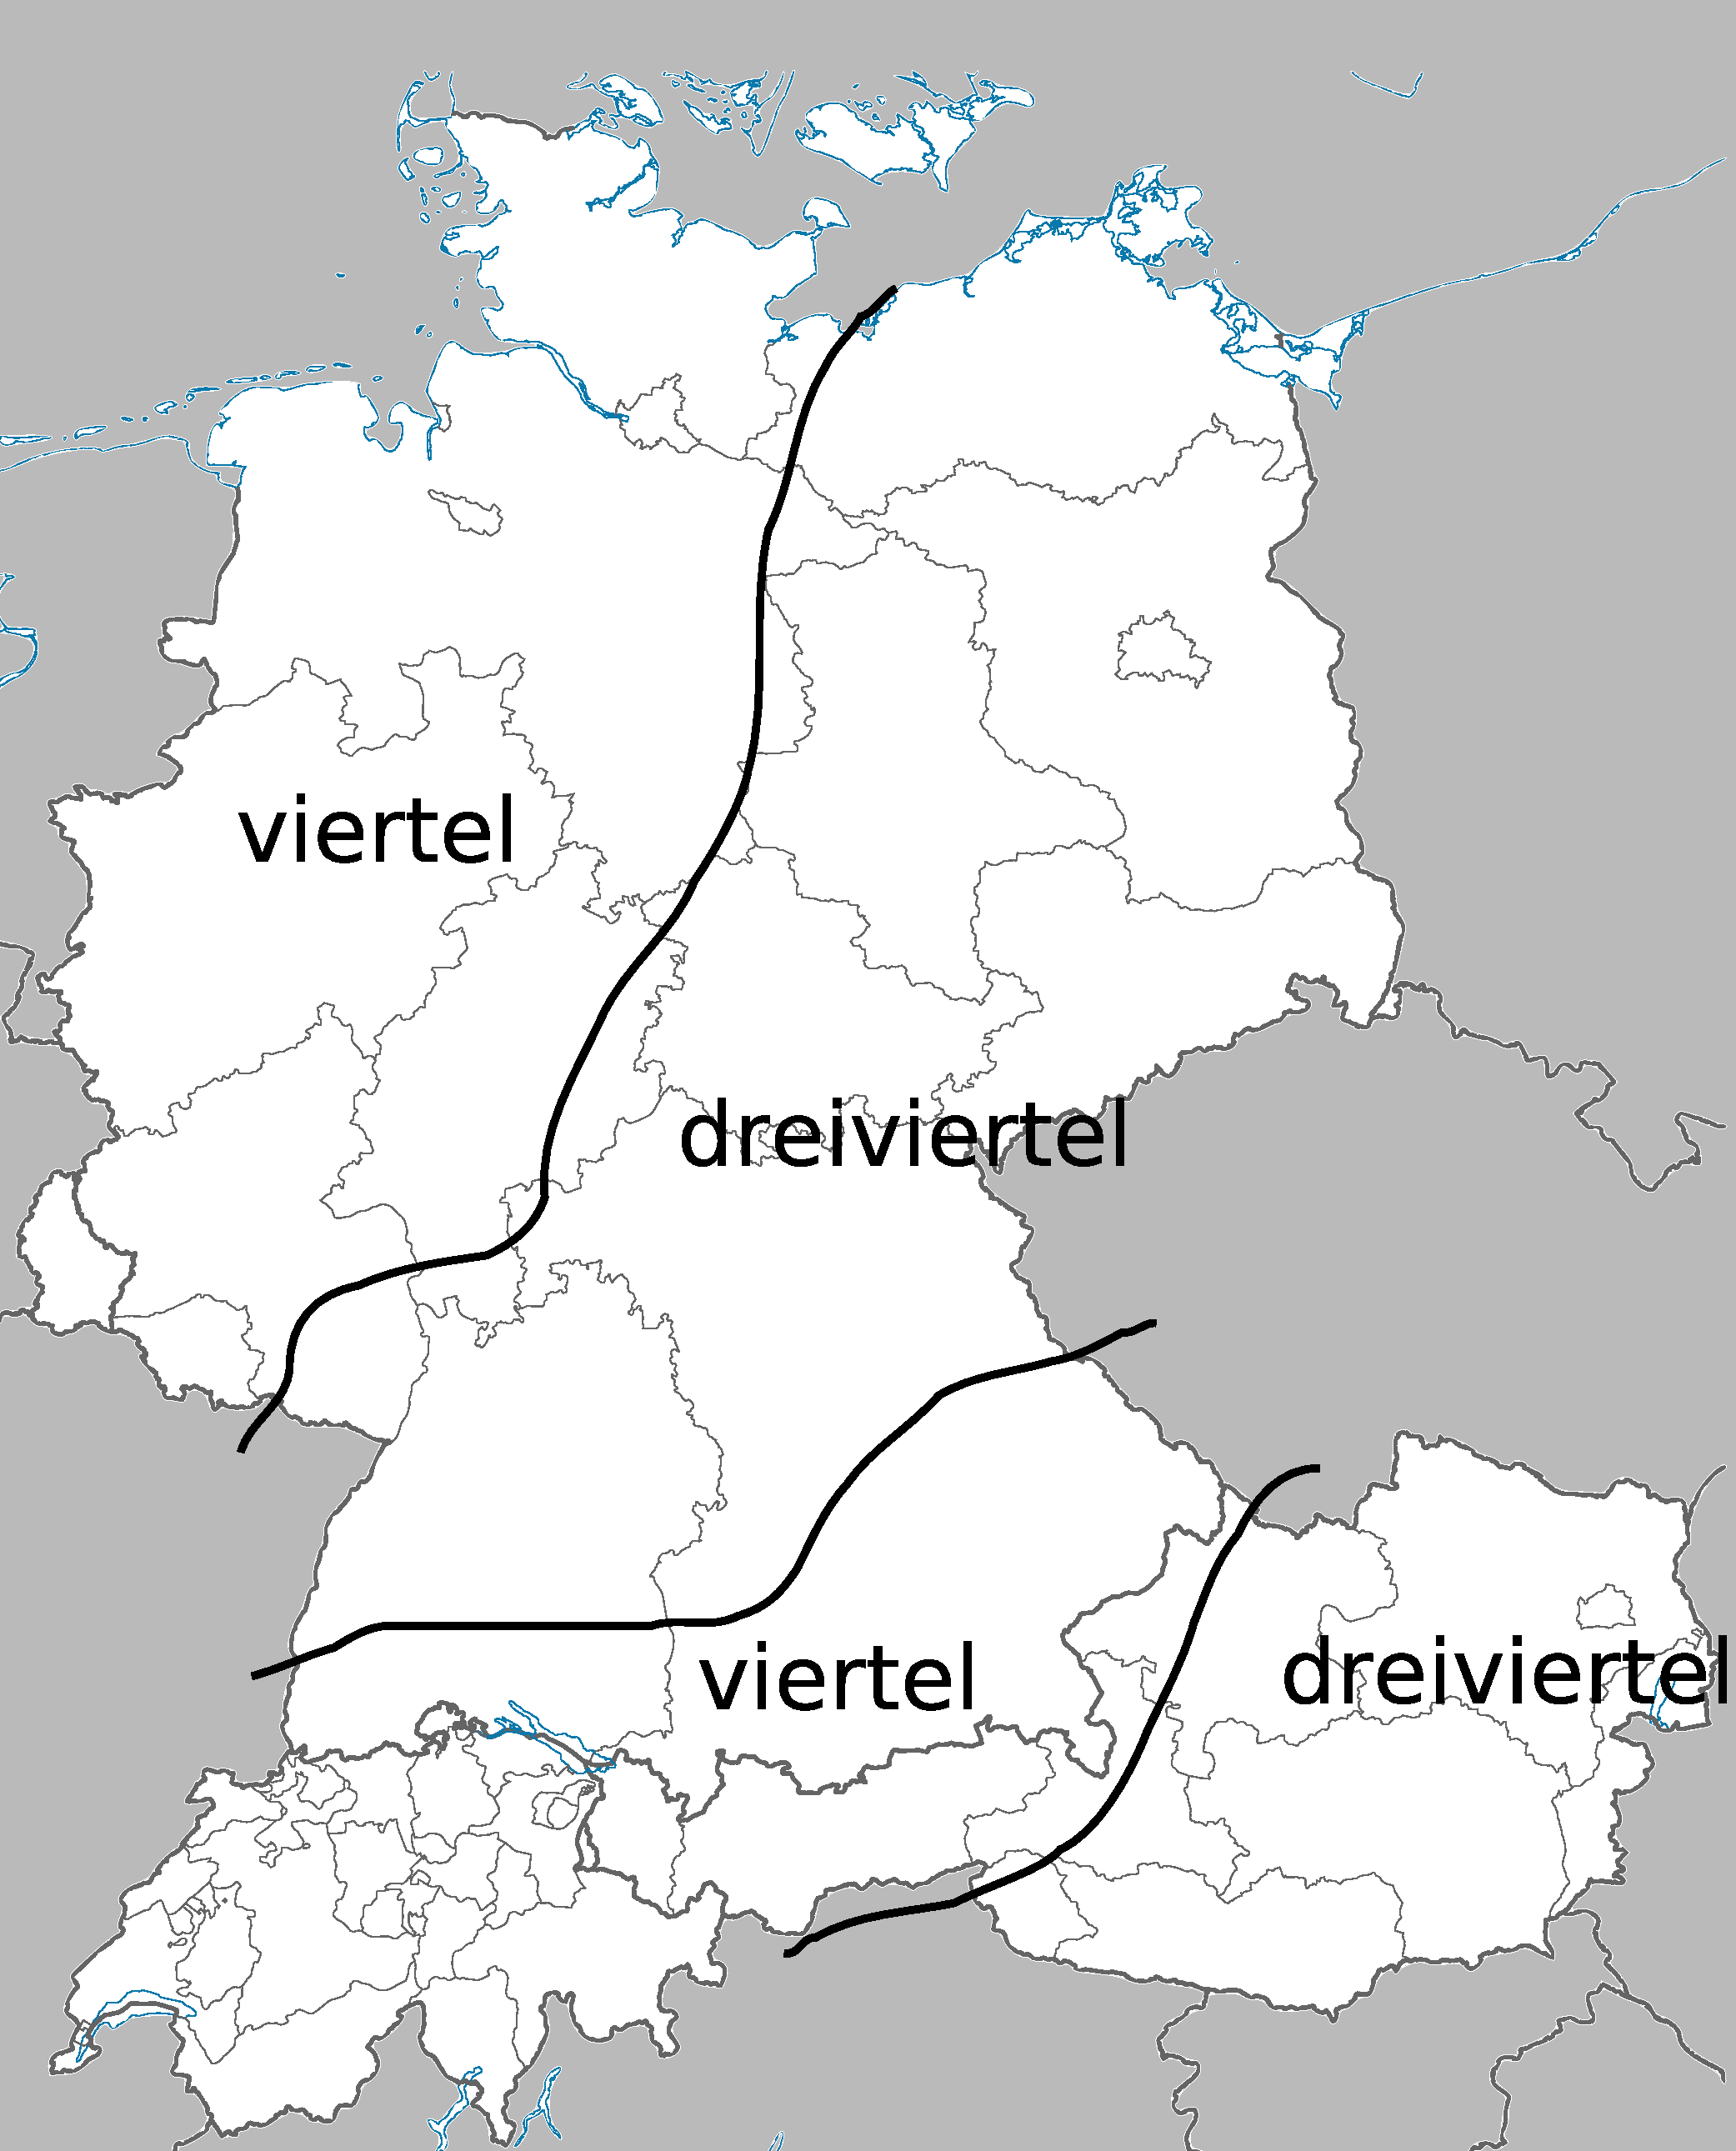
\includegraphics[width=1.00\textwidth]{regiomap.pdf}
	\label{fig:karte}
	\caption{Karte zur Verwendung von "`Dreiviertel"'}
\end{figure}
		
\clearpage
\section{Sicherung der Einstellungen}\label{sec_autoSave}
		Viele der vom Benutzer get�tigten Einstellungen 
		k�nnen gespeichert werden und bleiben auch nach einem 
		Stromausfall oder einem Trennen der Stromversorgung 
		erhalten. 
		
		Der Speichervorgang wird nach Bet�tigen der "`Ein/Aus"'-Taste durchgef�hrt.
		
		\ifthenelse{\WCautoSave=1}{
		  Au�erdem wird, wenn eine bestimmte Zeit kein Fernbedienungs-Kommando 
		  mehr empfangen wurde, automatisch eine Speicherung durchgef�hrt.
		}{}
		
		
		
		Zu den gesicherten Daten z�hlen: 
		\begin{compactitem}
				\item  antrainierte Fernbedienung 
				\item  vom Benutzer eingestellte Helligkeit 
				\item  ausgew�hlter Modus
        \ifthenelse{\WCindividualCfg=0 \or \WCmonocolor=0}{
					\item  ausgew�hltes Farbprofil 
					\item  Farbwerte der Farbprofile 
					\item  Farbwechsel-Geschwindigkeit 
				}{}
				\item  Puls-Geschwindigkeit 
				\item  gew�hltes Sprachprofil 
				\item  benutzerdefinierte Ein/Ausschaltzeiten 
		\end{compactitem}
		 
    \ifthenelse{\WCindividualCfg=0 \or \WCmonocolor=0}{
			\begin{Anmerkung}
					Das Speichern der per Hue-Farbwahl gew�hlten Farbe 
					funktioniert momentan noch nicht. 
			\end{Anmerkung}
		}{}



\end{document}